\chapter{Molecular Biology}\label{molecular-biology}

\href{https://en.wikipedia.org/wiki/Molecular_biology}{Molecular
biology} concerns the molecular basis of biological activity between
biomolecules in the various systems of a cell, including the
interactions between DNA, RNA, and proteins and their biosynthesis, as
well as the regulation of these interactions.

One of the most basic techniques of molecular biology to study protein
function is molecular cloning. In this technique, DNA coding for a
protein of interest is cloned using polymerase chain reaction (PCR),
and/or restriction enzymes into a plasmid (expression vector). A vector
has 3 distinctive features: an origin of replication, a multiple cloning
site (MCS), and a selective marker usually antibiotic resistance.
Located upstream of the multiple cloning site are the promoter regions
and the transcription start site which regulate the expression of cloned
gene. This plasmid can be inserted into either bacterial or animal
cells. Introducing DNA into bacterial cells can be done by
transformation via uptake of naked DNA, conjugation via cell-cell
contact or by transduction via viral vector. Introducing DNA into
eukaryotic cells, such as animal cells, by physical or chemical means is
called transfection. Several different transfection techniques are
available, such as calcium phosphate transfection, electroporation,
microinjection and liposome transfection. The plasmid may be integrated
into the genome, resulting in a stable transfection, or may remain
independent of the genome, called transient transfection.

DNA coding for a protein of interest is now inside a cell, and the
protein can now be expressed. A variety of systems, such as inducible
promoters and specific cell-signaling factors, are available to help
express the protein of interest at high levels. Large quantities of a
protein can then be extracted from the bacterial or eukaryotic cell. The
protein can be tested for enzymatic activity under a variety of
situations, the protein may be crystallized so its tertiary structure
can be studied, or, in the pharmaceutical industry, the activity of new
drugs against the protein can be studied.

\section{DNA restriction digest}\label{dna-restriction-digest}

\href{https://en.wikipedia.org/wiki/Lambda_phage}{Lambda DNA} comes from
a virus
(\href{https://en.wikipedia.org/wiki/Bacteriophage}{bacteriophage}) that
infects bacteria. This virus does not infect humans and is therefore
safe source to work with. Lambda DNA is approximately 48,000 base pairs
long.

When restriction enzymes are used to cut DNA fragments of varying sizes
are produced. Cut DNA can be separated using a process known as
\href{https://en.wikipedia.org/wiki/Agarose_gel_electrophoresis}{agarose
gel electrophoresis}. Agarose gel electrophoresis separates DNA
fragments by molecular weight. DNA fragments are loaded into an agarose
gel slab, which is placed into a chamber filled with a conductive buffer
solution. A direct current is passed between positive (red) and negative
(black) wire electrodes at each end of the chamber. DNA fragments are
negatively charged, and when placed in an electric field will be drawn
toward the positive pole (red). The matrix of the agarose gel acts as a
molecular sieve through which smaller DNA fragments can move more easily
than larger ones. Therefore, the distance and rate at which DNA
fragments migrate through the gel is inversely proportional to its
molecular weight. Over a period of time smaller fragments will travel
farther than larger ones. Fragments of the same size stay together and
migrate in discrete ``bands''.

\section{Preparing a gel for agarose gel
electrophoresis}\label{preparing-a-gel-for-agarose-gel-electrophoresis}

We will use gel electrophoresis to separate the DNA fragments obtained
from the restriction digest (Figure \ref{fig:box}). Before setting up
the digest, we will pour agarose gel because it will take about half an
hour for the gel to harden.

\begin{figure}

{\centering 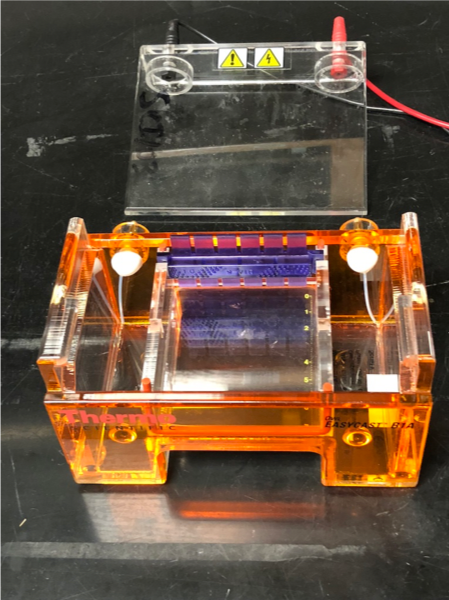
\includegraphics[width=0.7\linewidth]{./figures/molbio/Gel_box}

}

\caption{Agarose gel box with comb in place, ready for gel to be poured.}\label{fig:box}
\end{figure}

\subsection{Experimental procedures}\label{experimental-procedures-29}

\begin{enumerate}
\def\labelenumi{\arabic{enumi}.}
\setcounter{enumi}{1}
\tightlist
\item
  Get the Erlenmeyer flask containing 0.5 g of agarose powder
\item
  Add 50 ml of 1× TAE (Tris base, acetic acid, EDTA) running buffer.
\item
  Add 5 µl of SybrGreen™ dye (10,0× stock solution).
\item
  Heat in the microwave at full power for 1 minute.
\item
  Swirl to make sure that all powder has dissolved, and the solution is
  clear.
\item
  Add the comb into the comb slot.
\item
  Pour the solution onto the gel tray in the gel box.
\end{enumerate}

\section{Setting up the restriction digest
reactions}\label{setting-up-the-restriction-digest-reactions}

In this experiment, we will use three
\href{https://en.wikipedia.org/wiki/Restriction_enzyme}{restriction
enzymes} (EcoRI, Hind III, and Pst I) to cut Lambda DNA.

\subsection{Experimental procedures}\label{experimental-procedures-30}

\begin{enumerate}
\def\labelenumi{\arabic{enumi}.}
\tightlist
\item
  Digest DNA: microtubes that contain the enzyme stock solution, Lambda
  DNA, and restriction buffer are provided on ice (in an ice bucket).
\item
  Get 4 new microtubes and label each as follows:

  \begin{itemize}
  \tightlist
  \item
    Tube 1: L = Lambda DNA
  \item
    Tube 2: P = Pst I digest
  \item
    Tube 3: E = EcoRI digest
  \item
    Tube4: H = Hind III digest
  \end{itemize}
\item
  Use a new pipette tip for each transfer and pipet the reagents (from
  the stock solutions kept on ice) into each tube according to Table
  \ref{tab:digest}.
\item
  Mix the components by gently flicking the tube with your finger. Pulse
  spin the tubes in the microcentrifuge to collect all the liquid to the
  bottom of the tube.
\item
  Place the tubes in the heat block and incubate for 30 minutes at 37 °C.
\end{enumerate}

\begin{longtable}[]{@{}cccccc@{}}
\caption{\label{tab:digest} DNA digestion.}\tabularnewline
\toprule
Tube & DNA & buffer & Pst I & EcoR I & Hind III\tabularnewline
\midrule
\endfirsthead
\toprule
Tube & DNA & buffer & Pst I & EcoR I & Hind III\tabularnewline
\midrule
\endhead
L & 4 µl & 6 µl & \_ & \_ & \_\tabularnewline
P & 4 µl & 5 µl & 1 µl & \_ & \_\tabularnewline
E & 4 µl & 5 µl & \_ & 1 µl & \_\tabularnewline
H & 4 µl & 5 µl & \_ & \_ & 1 µl\tabularnewline
\bottomrule
\end{longtable}

\section{Loading the DNA samples on the agarose gel and agarose gel
electrophoresis}\label{loading-the-dna-samples-on-the-agarose-gel-and-agarose-gel-electrophoresis}

\begin{enumerate}
\def\labelenumi{\arabic{enumi}.}
\tightlist
\item
  Remove the digested DNA samples from the heat block.
\item
  Pulse spin the tubes in the centrifuge to bring all of the liquid to
  the bottom of the tube.
\item
  Add 2 µl of sample loading dye into each tube. Mix the contents by
  flicking the tube with your finger.
\item
  Fill the electrophoresis chamber and cover the gel with 1× TAE running
  buffer (this will require about 275 ml of buffer).
\item
  Check that the wells of the agarose gels are near the black (-)
  electrode and the base of the gel is near the red (+) electrode.
\item
  Load 12 µl of each sample into separate wells in the gel chamber in
  the following order:

  \begin{itemize}
  \tightlist
  \item
    Lane 1: L
  \item
    Lane 2: P
  \item
    Lane 3: E
  \item
    Lane 4: H
  \item
    Lane 5: DNA size marker
  \end{itemize}
\item
  Place the lid on the electrophoresis chamber. Connect the electrical
  leads into the power supply, red to red and black to black.
\item
  Turn on the power and run the gel at 120 V for 35 minutes (Figure
  \ref{fig:power}).
\end{enumerate}

\begin{figure}

{\centering 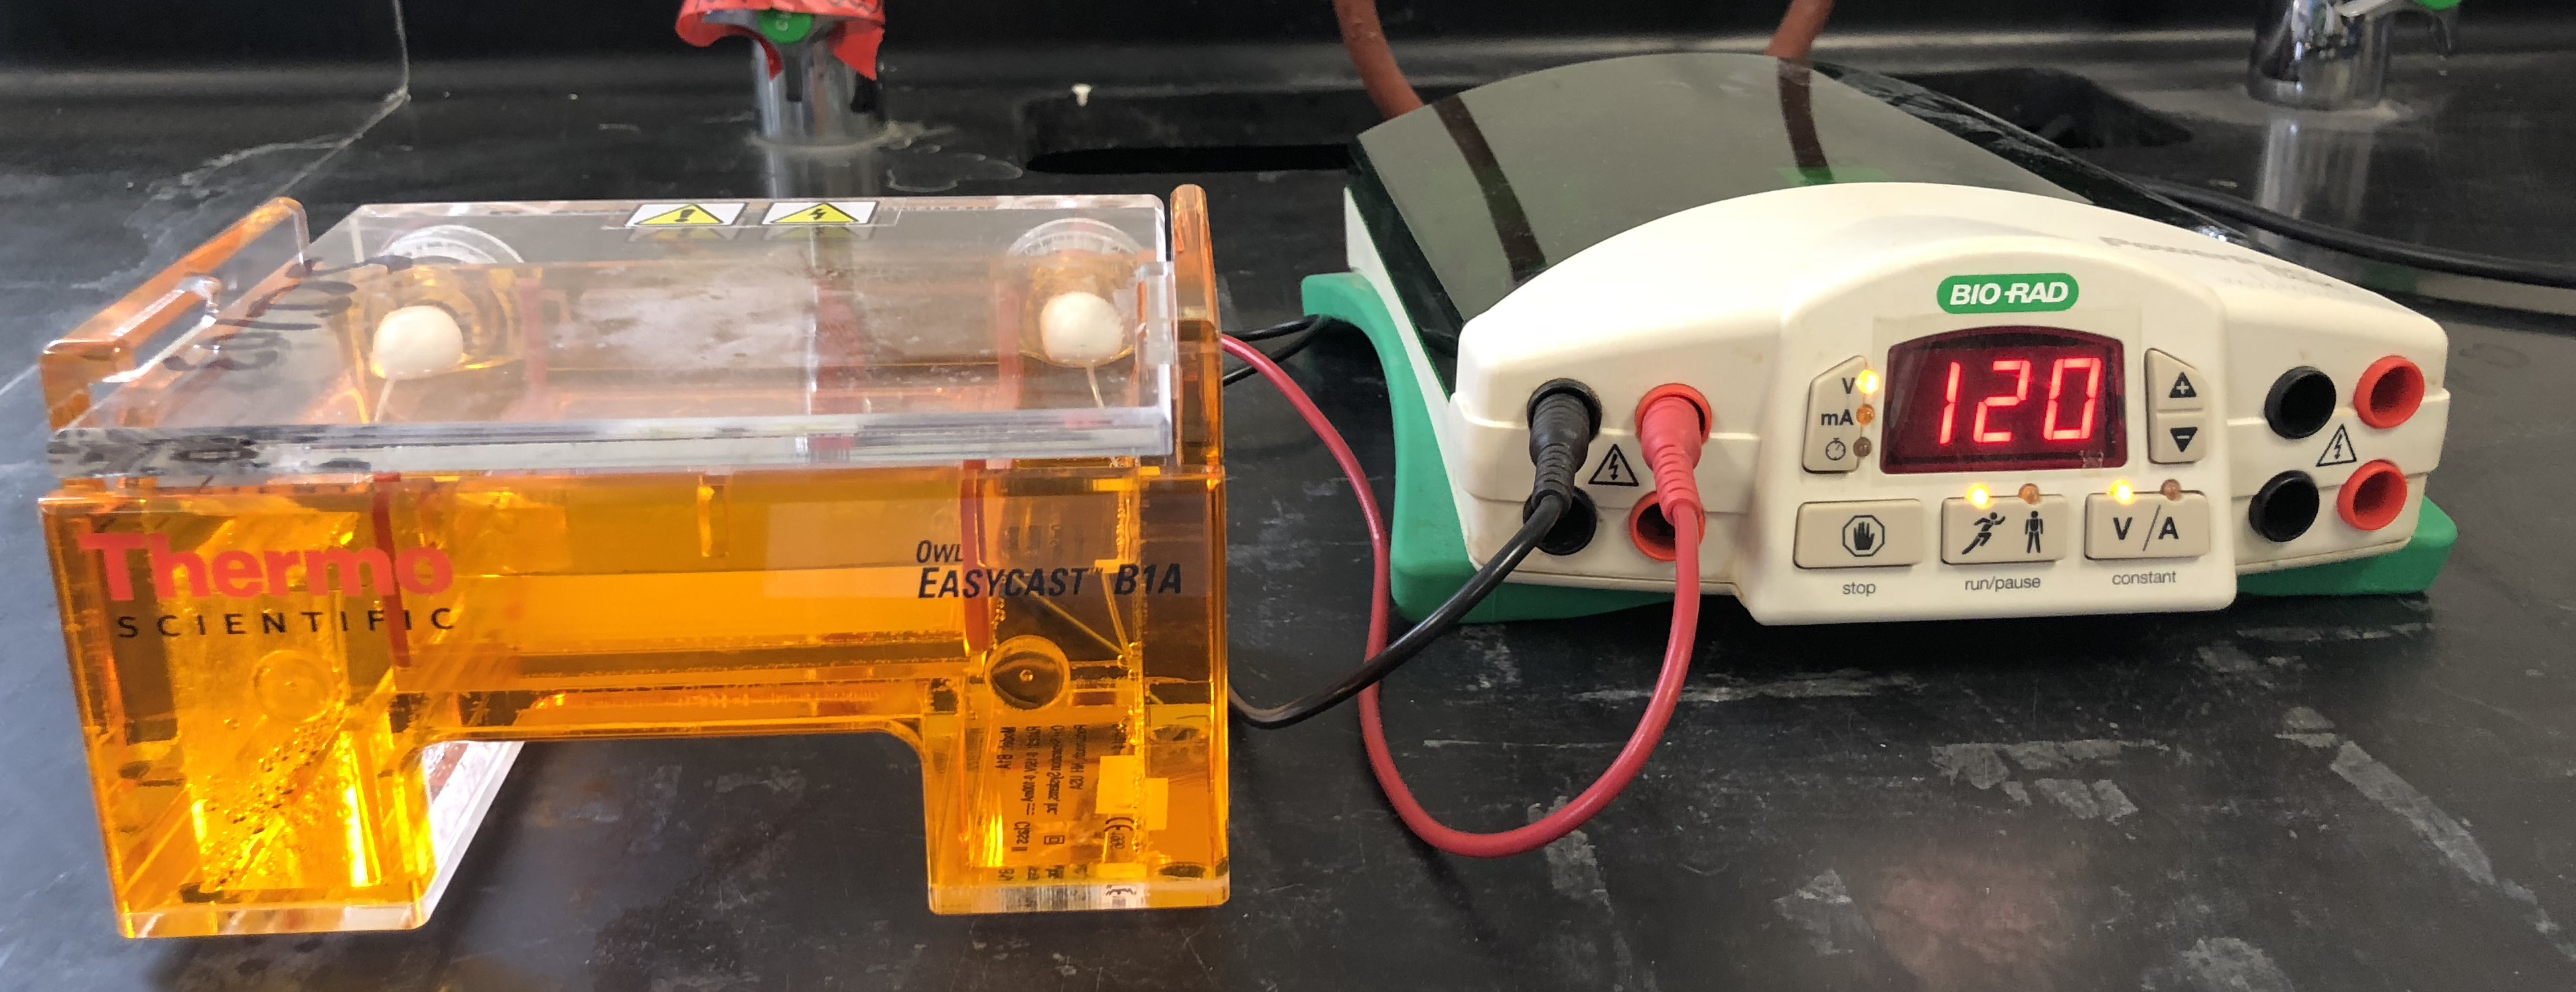
\includegraphics[width=0.7\linewidth]{./figures/molbio/Power_supply}

}

\caption{Gel electrophoresis box and power supply.}\label{fig:power}
\end{figure}

\section{Visualizing the DNA fragments from the restriction
digest}\label{visualizing-the-dna-fragments-from-the-restriction-digest}

We added a non-toxic green fluorescent dye to the agarose before we
poured the gel. The inclusion of this dye will allow us to visualize the
separated DNA fragments by exposing the gel to UV light source in the UV
light box (Figure \ref{fig:doc}).

\subsection{Experimental procedures}\label{experimental-procedures-31}

\begin{enumerate}
\def\labelenumi{\arabic{enumi}.}
\tightlist
\item
  Visualize cut DNA using the UV light box (Figure \ref{fig:doc}).
\item
  Print out a picture of the gel.
\end{enumerate}

\begin{figure}

{\centering 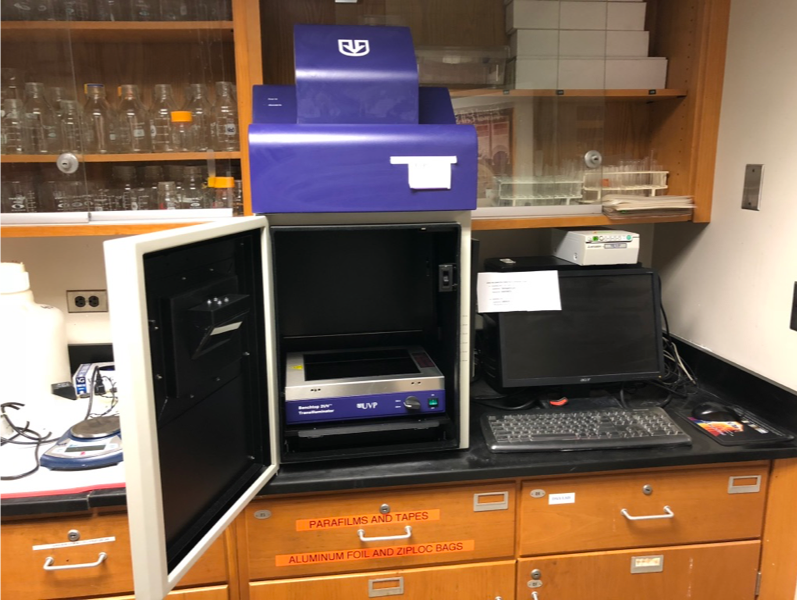
\includegraphics[width=0.7\linewidth]{./figures/molbio/Gel_doc}

}

\caption{Gel documentation system with UV light source.}\label{fig:doc}
\end{figure}

\section{Review Questions}\label{review-questions-8}

\begin{enumerate}
\def\labelenumi{\arabic{enumi}.}
\tightlist
\item
  What is DNA made of?
\item
  What is a restriction enzyme?
\item
  What is a DNA ligase?
\item
  What is a DNA polymerase?
\item
  What is molecular cloning?
\item
  What is gel electrophoresis?
\item
  In an electric field, DNA moves from the \underline{\phantom{answer}} to
  the \underline{\phantom{answer}} pole.
\item
  Smaller fragments of DNA move \underline{\phantom{answer}} than larger
  fragments.
\end{enumerate}
